\subsection{Physical Structure}
The structure of the robot should allow the movement of the robot across the map. 
That means, the robot should have at least two motors to move in the plane of the circuit and a minimum of two light sensors to check its position referred to the black lines of the map and check when the robot has arrived to a crossroad.

The chosen motor configuration consist in the use of two motors that move two parallel wheels. 
This allows the robot to change the direction of the movement setting a different motor speed on each motor.

\todo[inline]{support? using the 3rd line sensor.}

Two light sensors are used as seen in figure \ref{fig:robotscheme}. 
In the position control, the value of the sensors are compared and the robot is controlled having in mind that the value of the sensors should be the same when the robot is centred above the line.
When the value of both sensors are low, the robot is facing a crossroad.

The position of the light sensors is in the front of the robot, and the distance between them should be enough to correctly detect the line. 
This means the light sensors should be placed close to the edges of the line such that they both detect a part of the line.
Because of that the distance between them should be around the width of the line itself as shown in figure \ref{fig:robotscheme}.

\todo[inline]{sensor offset? variability? stability?}

\begin{figure}[H]
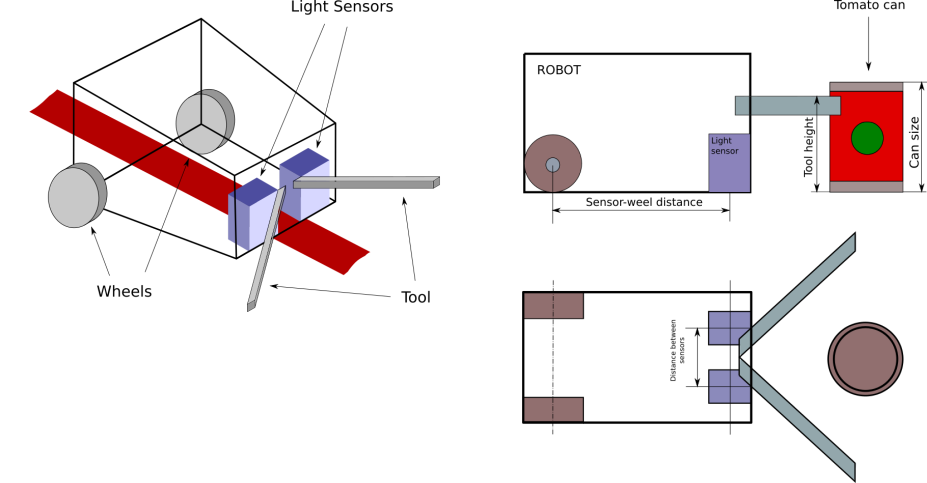
\includegraphics[width=10cm]{Fig2.png}
\centering
\caption{Scheme of the proposed configuration.}
\label{fig:robotscheme}
\end{figure}


To be able to push and guide the can across the map, the robot should have a proper tool that allows this task. 
The proposed design consist of two bars placed making an angle that allows the guide of the bottle when driving straight forward, as is shown in figure \ref{fig:robotscheme}.
This configuration allows catching the can even when its position is displaced, making the robot's job more easy.

Considering the rules of the game then the can is not permitted to be pushed left or right and because of that, no special design enabling this are required. 
The turning back behaviour is more difficult. 
%As the distance between the lines are short, the turn back should be done in a small place because the sensors should find the line before the crossroad.
The distance between the line intersections are short and the turn back has to happen in free space without interacting with the nearby placed cans.
At the same time, the robot should also finish the turn before reaching the new intersection, so the full length of the robot should be short enough to allow these movements.


The final build of the robot is seen in figure \ref{fig:robotImage}.

\begin{figure}[H]
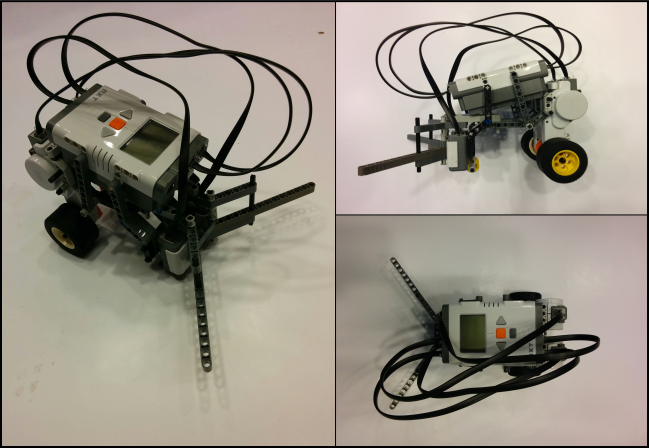
\includegraphics[width=10cm]{Fig1.png}
\centering
\caption{Images of the built robot.}
\label{fig:robotImage}
\end{figure}